\chapter{Structure globale}


\section{Le projet en général}

\begin{figure}[h]
\begin{center}
	\makebox[\textwidth]{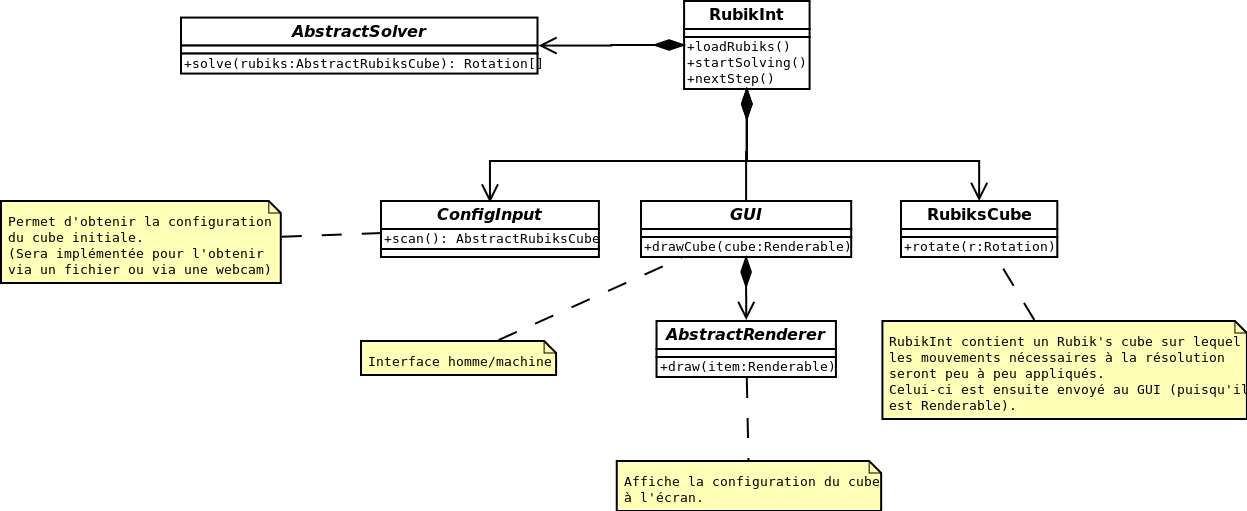
\includegraphics[width=.8\paperwidth]{diagrammes/projet.png}}
\end{center}
\caption{GUI}
\end{figure}

Nous avons décidé de découper notre projet en plusieurs classes.
La classe principale de notre application est \textit{RubikInt}.
Celle-ci possède trois classes: l'interface graphique (ici noté \textit{GUI}), l'objet stockant la configuration du RubiksCube et celui en charge de charger la configuration et créer une instance de \textit{RubiksCube}.
La classe principale utilise également un résolveur qui recherchera les mouvements pour résoudre le cube.

\section{L'object Rubik's Cube}

\begin{figure}[h]
\begin{center}
	\makebox[\textwidth]{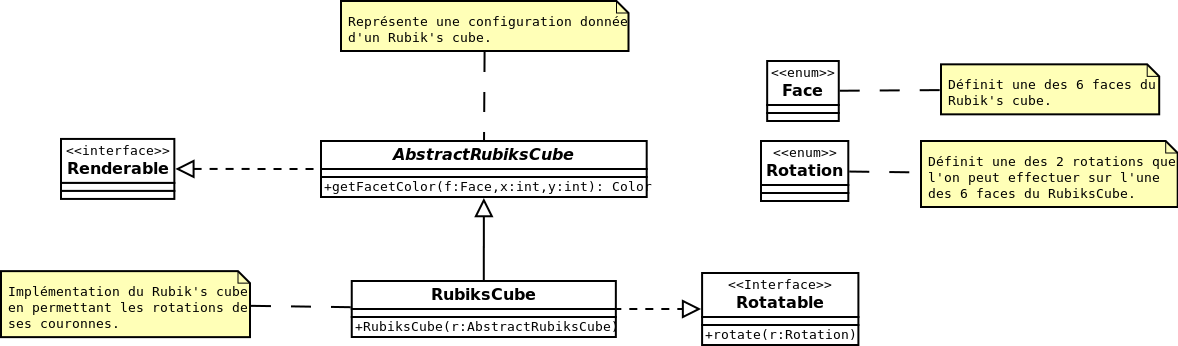
\includegraphics[width=.8\paperwidth]{diagrammes/rubikscube.png}}
\end{center}
\caption{GUI}
\end{figure}

Nous avons créé une classe abstraite pour permettre de multiples implémentations du Rubik's.
Un RubiksCube est "\textit{Rotatable}" et "\textit{Renderable}", il hérite donc de ces interfaces qui définissent son comportement.

